\chapter{Prospects on differential \textsl{t}-channel measurements at 13~TeV}
\label{ch:prospects}

\intro{Prospects on extending the presented measurement in Ch.~\ref{ch:diff13} are discussed. This study uses \gls{pp} collision data corresponding to 36~\invfb which were recored with the \gls{cms} experiment in 2016. Potential improvements in the training of \acrlongpl{bdt}, the fitting procedure, and in the unfolding are demonstrated. In particular, the measurement of differential cross sections at particle level is envisaged. The presented technical study of object definition and event selection at particle level for $t$-channel single-top-quark events has been published in Ref.~\cite{particleStudies}. }

\todo{update note ref}

%##############################################
\section{Setup}
%##############################################

The analysis strategy which has been developed in the context of the first measurement of differential cross section of $t$-channel single-top-quark-production (Ch.~\ref{ch:diff13}) is extended as follows. The data statistics is increased by using \gls{pp} collision data recored in 2016 with the \gls{cms} detector at a \acrlong{cm} energy of 13~\TeV corresponding to 36~\invfb. Events containing an isolated muon candidate and two or three jets are selected using mostly the criteria detailed in Sec.~\ref{sec:diff13-selection} with a few exceptions as outlined in the following. Due to the higher instantaneous luminosity in the 2016 data-taking period compared to 2015 which peaked at $15.3~\mathrm{Hz}/\mathrm{nb}$~\cite{lumipublic}, the threshold of the employed single muon trigger has been raised to $24~\GeV$. Consequently, muon candidates with a higher threshold of $\pt>26~\GeV$ are required offline as well. All other muon selection criteria are kept the same. The analysis of events containing single electrons and two or three jets is also envisaged for a potential update of the differential cross section measurement. Corresponding data events are recorded with an electron trigger that requires an electron candidate with a transverse momentum of at least $32~\GeV$ within $|\eta|<2.1$. Offline, events must contain a corresponding electron candidate with $\pt>35~\GeV$ within $|\eta|<2.1$. The candidate has to fulfill furthermore tight identification criteria which have been specifically designed to select most genuine electrons~\cite{CMS-DP-2017-004}.

For b-tagging a new algorithm, the so-called \gls{cmva}-tagger (combined MVA)~\cite{CMS-PAS-BTV-15-001} is employed which includes amongst others the output of the previously used \gls{csv} algorithm in its training as well. At its tight working point an efficiency of about 55\% is obtained for true b~jets which is approximately 5\% higher than the efficiency of the \gls{csv} algorithm while both algorithms have a mistagging rate of only 0.1\% for light-flavored jets originating from u,d,s quarks and gluons.

The remainder of the event selection is kept identical to Sec.~\ref{sec:diff13-selection} which concerns the veto of events containing additional leptons, the jet clustering, and the categorization of events into signal and control regions based on the number of selected jets and b-tags.

The following samples of simulated events are used for this study. A sample of single-top-quark $t$-channel events has been generated with the \POWHEG generator interfaced with \PYTHIA{}8 and \MADSPIN. The \POWHEG generator interfaced with \PYTHIA{}8 is also used to generated events of tW single-top-quark and \ttbar production. Samples of \wjets and \zjets production are generated with the \MGAMC generator interfaced with \PYTHIA{}8. Exclusive \wjets samples with zero, one, or two extra jets are generated and merged with the \gls{fxfx} procedure~\cite{Frederix:2012ps}. The cross sections for normalizing these samples are identical to the ones used in Ch.~\ref{ch:diff13} and can be found in Tab.~\ref{tab:diff13-theo-xsecs} with the exception of the exclusive \wjets cross sections which are listed in Tab.~\ref{tab:prospects-theo-xsecs} instead.

\mytable{\label{tab:prospects-theo-xsecs}Theoretical \gls{sm} cross sections used to normalize the exclusive \wjets samples.}{
\begin{tabular}{@{}l  r c l@{}}
\toprule
$\mathrm{W}\to\ell\nu\mathrm{\,\mbox{+}\,0~jets}$ & $49\,670~\pb$ && \gls{nlo} \hfill (reported by \MGAMC) \\
$\mathrm{W}\to\ell\nu\mathrm{\,\mbox{+}\,1~jet}$ & $8\,264~\pb$ && \gls{nlo} \hfill (reported by \MGAMC) \\
$\mathrm{W}\to\ell\nu\mathrm{\,\mbox{+}\,2~jets}$ & $2\,544~\pb$ && \gls{nlo} \hfill (reported by \MGAMC) \\
\bottomrule
\end{tabular}
}


The contamination by multijet events are estimated in muon and electron channel through templates extracted from data in a sideband region. In the muon channel, the sideband region is defined by inverting the relative isolation as $\muiso>20\%$. In the electron channel on the other hand the isolation requirement is part of the used identification. Thus a sideband region is defined by vetoing the identification criteria. The resulting description of data by the multijet templates is validated in the 2j0t control region. In Fig.~\ref{fig:pospects-met-wjets} the \met distribution and the distribution of the $\phi$ angle between the lepton and the transverse momentum vector are presented for both channels after scaling the templates to the result of a \gls{ml} fit as detailed in Sec.~\ref{sec:prospects-fit}. The \met distributions display a good agreement between the data and predictions. A good description of data by the multijet template and the \wjets sample is also achieved for the $\Delta\phi(\mu,\met)$ distribution in the muon channel. In the electron channel a slight mismodeling is observed which may be mitigated by fine-tuning the sideband region further.


\myfigure[p]{\label{fig:pospects-met-wjets} Distributions of (top row)~the transverse missing energy and (bottom row)~the difference in $\phi$ angle between the lepton and the missing transverse energy in the 2j0t control region for (a)~electron and (b)~muon events.}{
\subfloat[]{\adjincludegraphics[height=4.8cm,trim={0 0 {0.16\width} 0},clip]{figures/prospects/plots/2j0t/electron_2j0t_met_qcdnone_nol.pdf}}
\subfloat[]{\adjincludegraphics[height=4.8cm,trim={0 0 {0.\width} 0},clip]{figures/prospects/plots/2j0t/muon_2j0t_met_qcdnone.pdf}}\\
\subfloat[]{\adjincludegraphics[height=4.8cm,trim={0 0 {0.16\width} 0},clip]{figures/prospects/plots/2j0t/electron_2j0t_lepton_met_deltaPhi_qcdnone_nol.pdf}}
\subfloat[]{\adjincludegraphics[height=4.8cm,trim={0 0 {0.\width} 0},clip]{figures/prospects/plots/2j0t/muon_2j0t_lepton_met_deltaPhi_qcdnone.pdf}}
}

\myfigure[p]{\label{fig:pospects-topmass} Distributions of the reconstructed top quark mass for (left column)~electron and (right column)~muon channel: (top row)~signal region; (bottom row)~\ttbar control region.}{
\subfloat[]{\adjincludegraphics[height=4.8cm,trim={0 0 {0.16\width} 0},clip]{figures/prospects/plots/2j1t/electron_2j1t_top_mass_qcdnone_nol.pdf}}
\subfloat[]{\adjincludegraphics[height=4.8cm,trim={0 0 {0.\width} 0},clip]{figures/prospects/plots/2j1t/muon_2j1t_top_mass_qcdnone.pdf}}\\
\subfloat[]{\adjincludegraphics[height=4.8cm,trim={0 0 {0.16\width} 0},clip]{figures/prospects/plots/3j1t/electron_3j1t_top_mass_qcdnone_nol.pdf}}
\subfloat[]{\adjincludegraphics[height=4.8cm,trim={0 0 {0.\width} 0},clip]{figures/prospects/plots/3j1t/muon_3j1t_top_mass_qcdnone.pdf}}
}






%##############################################
\section{New BDT training}
%##############################################

The following observables have been chosen as input to the \gls{bdt} training:

\begin{itemize}
\item the invariant mass of the reconstructed top quark candidate;
\item the missing transverse energy, \met;
\item the transverse momentum of the dijet system, $(\vec{p}_\mathrm{b}+\vec{p}_{\jprime})_\mathrm{T}$;
\item the event shape C as introduced in Sec.~\ref{sec:diff13-bdt};
\item the $\Delta R$ distance between the two jets;
\item the $\Delta R$ distance between the b-tagged jet and the lepton;
\item the invariant mass of the \acrlong{cm} system; $\sqrt{\hat{s}}=|p_\mathrm{top}+p_{\jprime}|$;
\item the W~boson helicity angle, defined between the top quark and lepton momentum in the W~boson rest frame (see Sec.~\ref{sec:theory-top-quark-decay} for details), $\cos\theta_\mathrm{W}^\star$;
\end{itemize}

In particular, the 

\myfigure[p]{\label{fig:prospects-cosWhel} Distributions of the W~boson helicity angle in 2j1t (a)~electron and (b)~muon channel.}{
\subfloat[]{\adjincludegraphics[height=4.8cm,trim={0 0 {0.16\width} 0},clip]{figures/prospects/plots/2j1t/electron_2j1t_cosTheta_wH_qcdnone_nol.pdf}}
\subfloat[]{\adjincludegraphics[height=4.8cm,trim={0 0 {0.\width} 0},clip]{figures/prospects/plots/2j1t/muon_2j1t_cosTheta_wH_qcdnone.pdf}}
}



\myfigure[p]{\label{fig:prospects-bdt-tt} Distributions of the \bdttt discriminant, trained to separate \ttbar from \wjets events, in 2j1t (a)~electron and (b)~muon channel.}{
\subfloat[]{\adjincludegraphics[height=4.8cm,trim={0 0 {0.16\width} 0},clip]{figures/prospects/plots/2j1t/electron_2j1t_bdt_ttw_boost04_CR_nol.pdf}}
\subfloat[]{\adjincludegraphics[height=4.8cm,trim={0 0 {0.\width} 0},clip]{figures/prospects/plots/2j1t/electron_2j1t_bdt_ttw_boost04_CR.pdf}}
}

\myfigure[p]{\label{fig:prospects-bdt-tch} Distributions of the \bdttch discriminant, trained to separate signal from \ttbar and \wjets events, in 2j1t (a)~electron and (b)~muon channel.}{
\subfloat[]{\adjincludegraphics[height=4.8cm,trim={0 0 {0.16\width} 0},clip]{figures/prospects/plots/2j1t/electron_2j1t_bdt_tch_boost04_qcdnone_blind_nol.pdf}}
\subfloat[]{\adjincludegraphics[height=4.8cm,trim={0 0 {0.\width} 0},clip]{figures/prospects/plots/2j1t/muon_2j1t_bdt_tch_boost04_qcdnone_blind.pdf}}
}

%##############################################
\subsection{Signal extraction}
%##############################################
\label{sec:prospects-fit}

%##############################################
\section{Fiducial studies}
%##############################################
\label{sec:prospects-fiducial-studies}



Figures~\ref{fig:prospects-particle-level-muonpt} and~\ref{fig:prospects-particle-level-muoneta} show a comparison of the muon $\pt$ and pseudorapidity at reconstruction, particle, and parton level after selecting events with one muon at each level respectively. The top panels demonstrate a high overlap of the events selected at reconstruction level with the ones at particle and parton level. The acceptance rises with the muon momentum from about 40\% to 90\% due to the relative isolation requirement for reconstructed muons. The number of jets is presented in Fig.~\ref{fig:prospects-particle-level-njet}. Due to the jet energy scale correction, 


dressed leptons (cone algorithms associates photons to leptons but does not cluster close leptons), tau decays, jet clustering (no neutrinos/leptons), b-tagging,




particle level overlap: tightMu: >99\%, 2jets: 80\%, 2j1t: 70\%


\myfigure[p]{\label{fig:prospects-particle-level}Comparison of expected event densities for $1~\invfb$ at $13~\TeV$ after applying the event selection at reconstruction, particle, and parton level respectively:  (a)~muon $\pt$, (b)~muon rapidity, and (c)~number of jets after requiring one isolated and tight muon; (d)~number of b-tagged jets, (e)~$\pt$ and (f)~pseudorapidity of the spectator jet after requiring one isolated, tight muon and two jets where in (e,f) one jet is additionally required to be b-tagged at reconstruction level. Top panels show the common events selected at reconstruction level while the bottom panels display the acceptance.}{
\subfloat[\label{fig:prospects-particle-level-muonpt}]{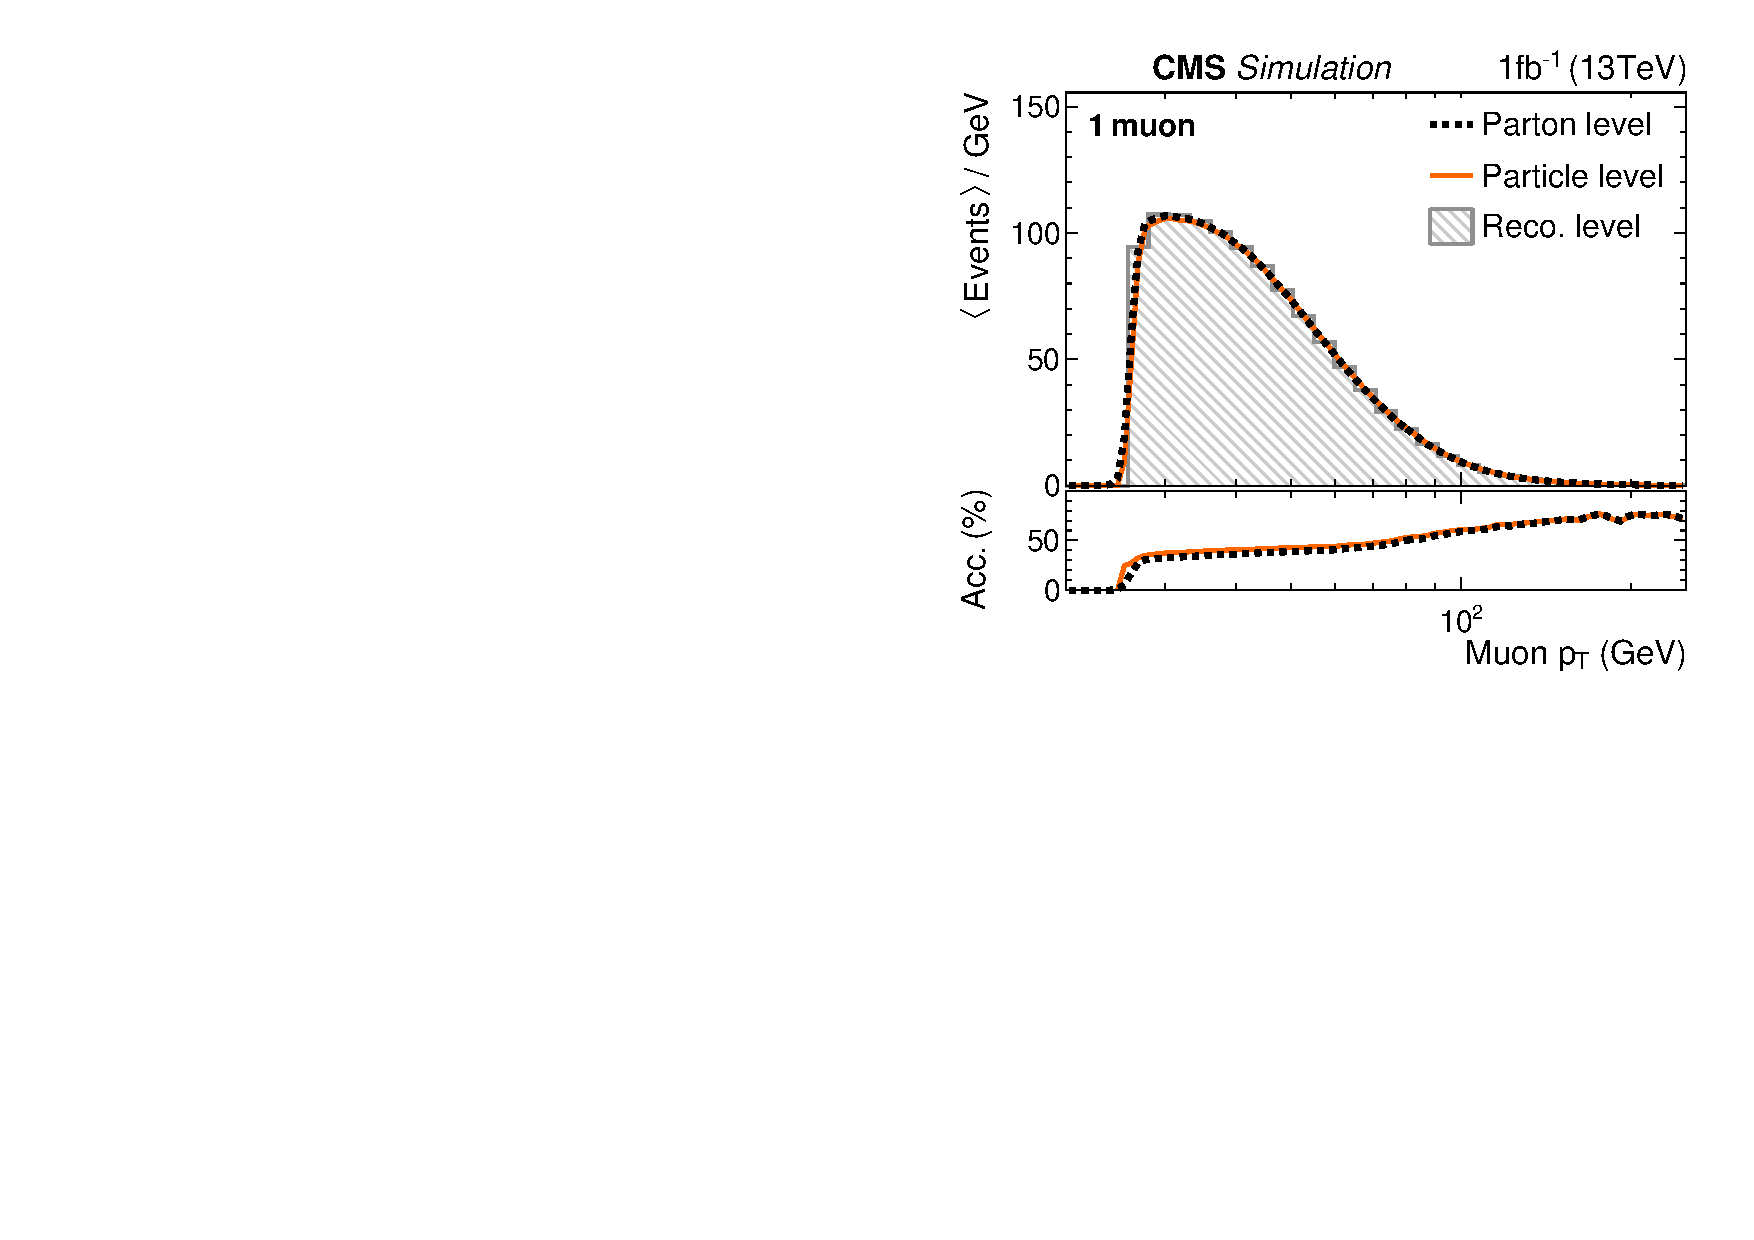
\includegraphics[width=0.48\textwidth]{figures/prospects/fiducial/muon_particle_logpt.pdf}}\hspace{0.03\textwidth}
\subfloat[\label{fig:prospects-particle-level-muoneta}]{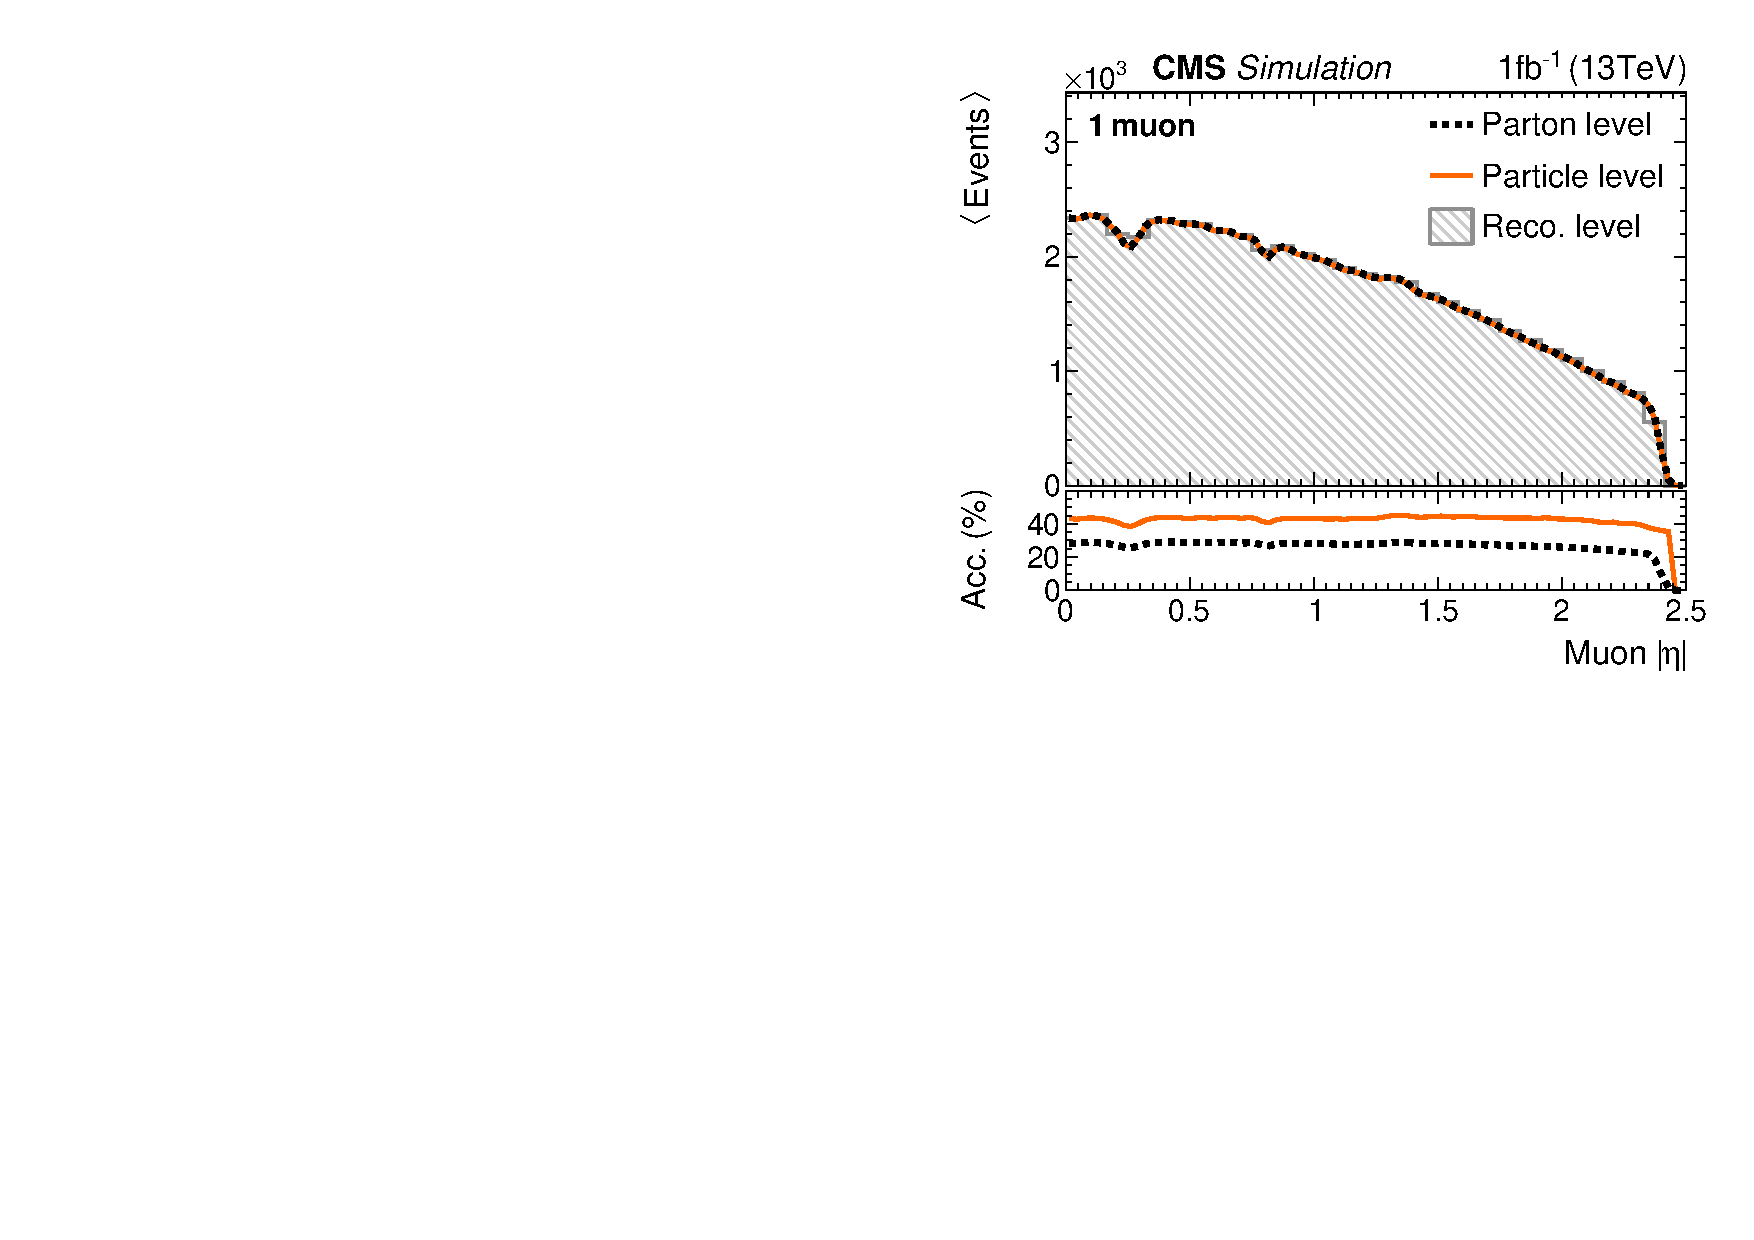
\includegraphics[width=0.48\textwidth]{figures/prospects/fiducial/muon_particle_abseta.pdf}}\\
\subfloat[\label{fig:prospects-particle-level-njet}]{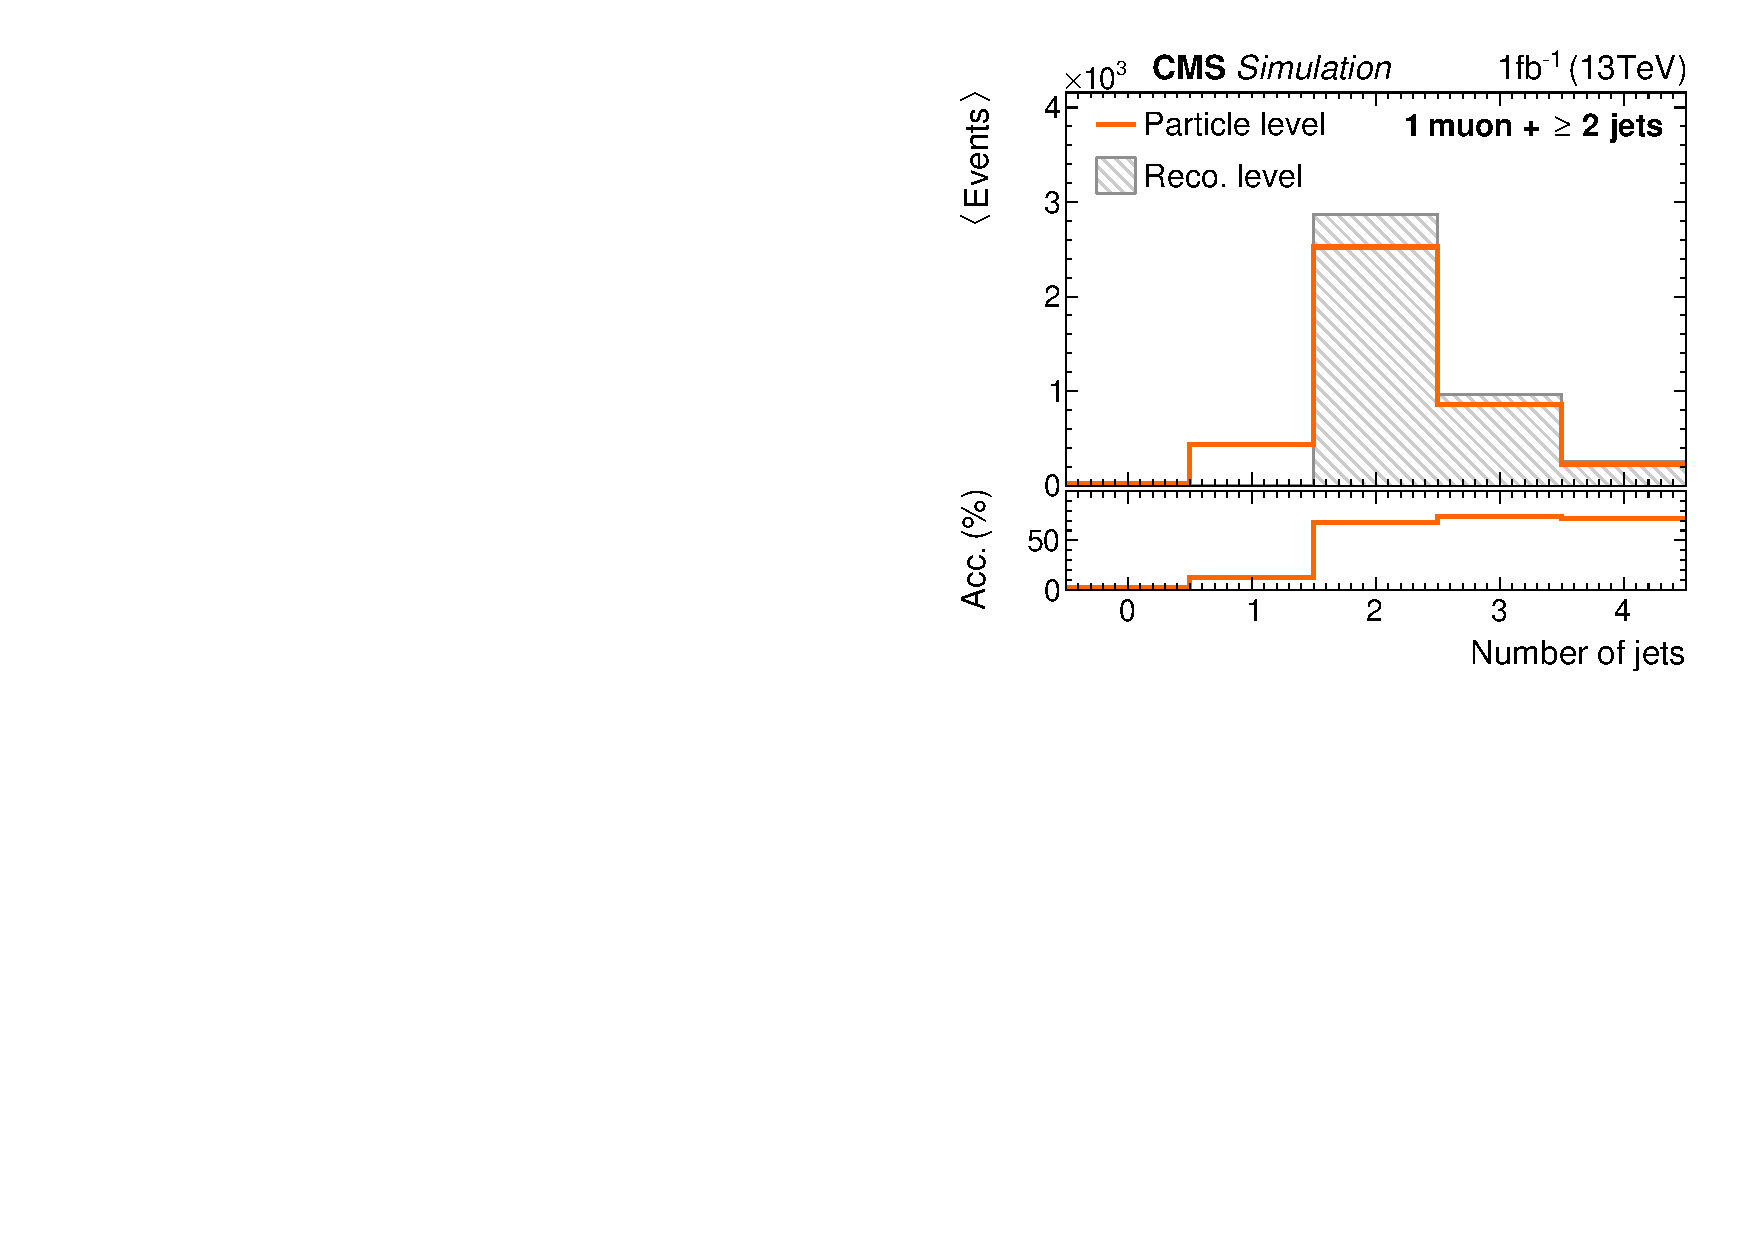
\includegraphics[width=0.48\textwidth]{figures/prospects/fiducial/njet_particle.pdf}}\hspace{0.03\textwidth}
\subfloat[\label{fig:prospects-particle-level-nbjet}]{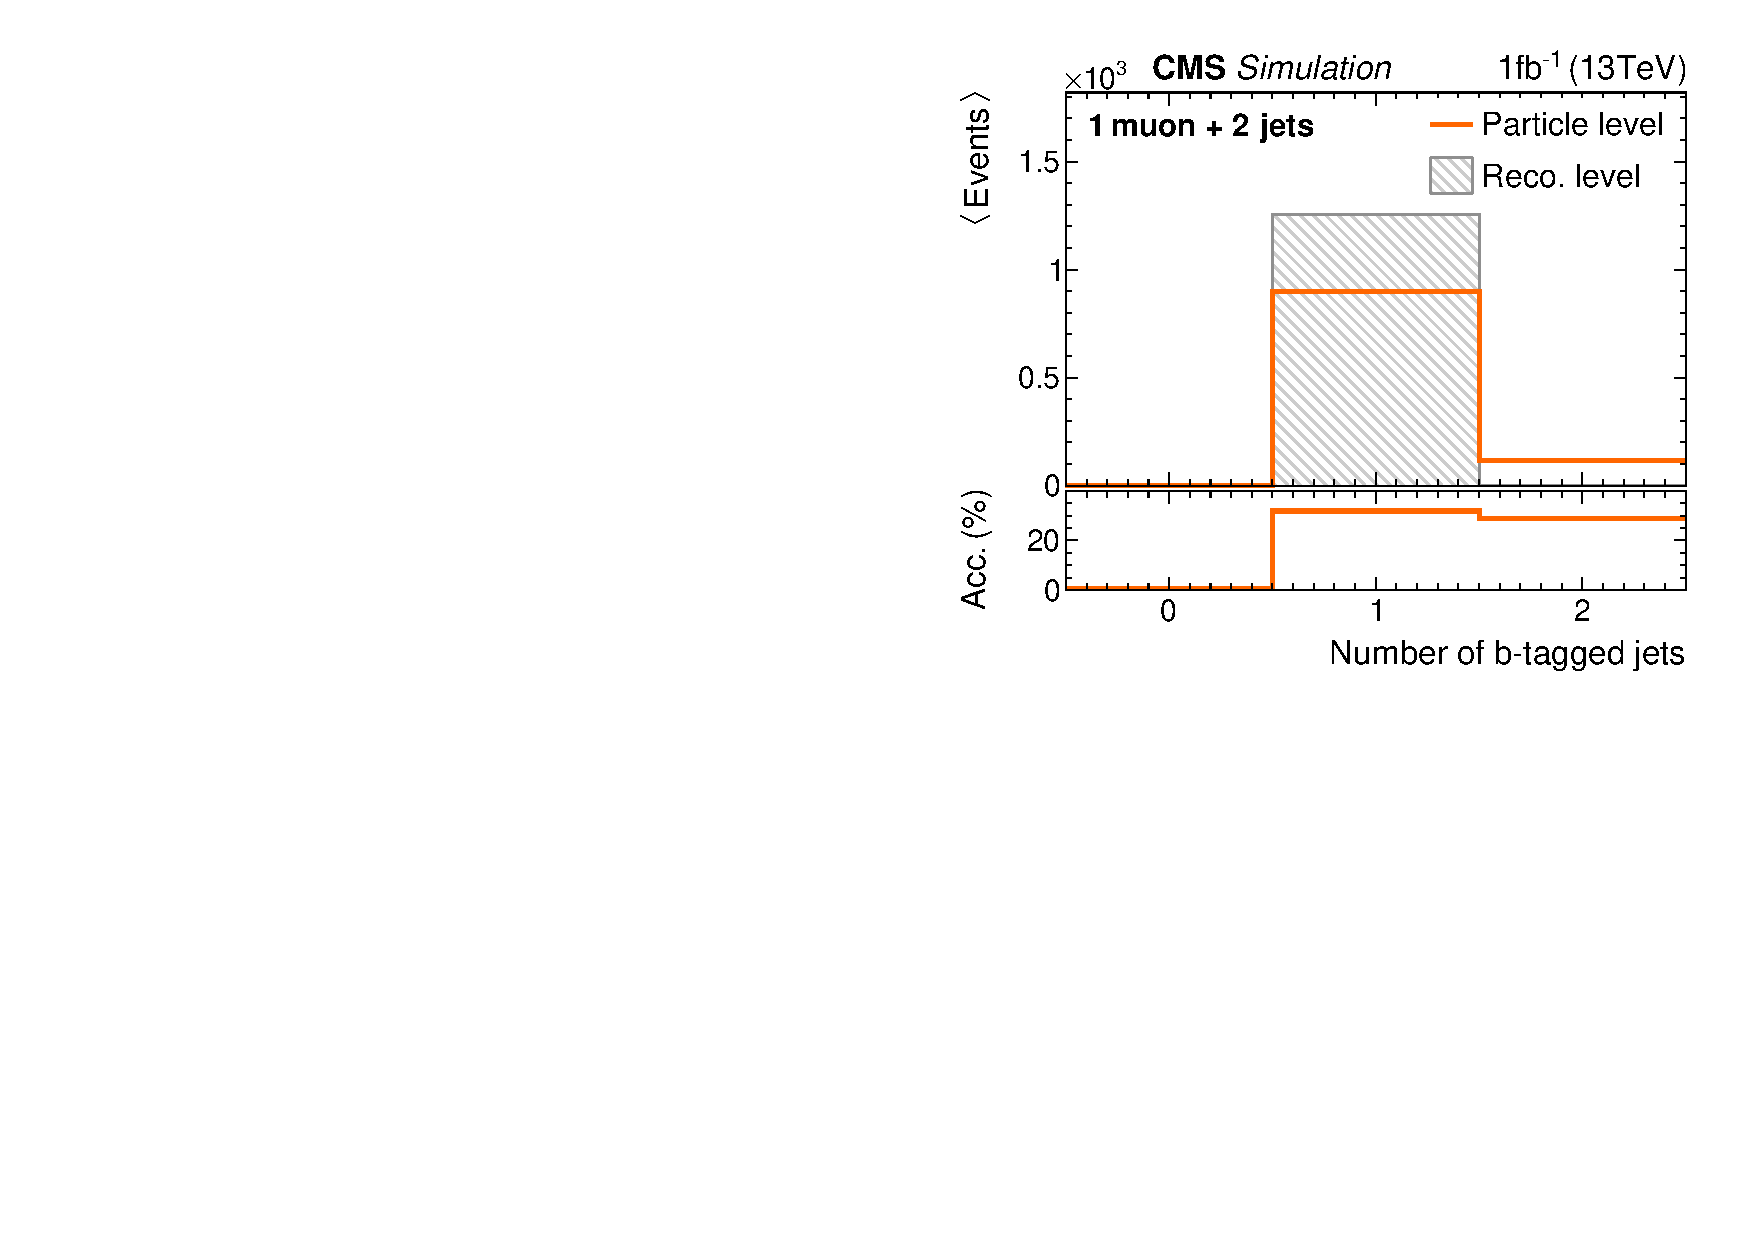
\includegraphics[width=0.48\textwidth]{figures/prospects/fiducial/nbjet_particle.pdf}}\\
\subfloat[\label{fig:prospects-particle-level-ljetpt}]{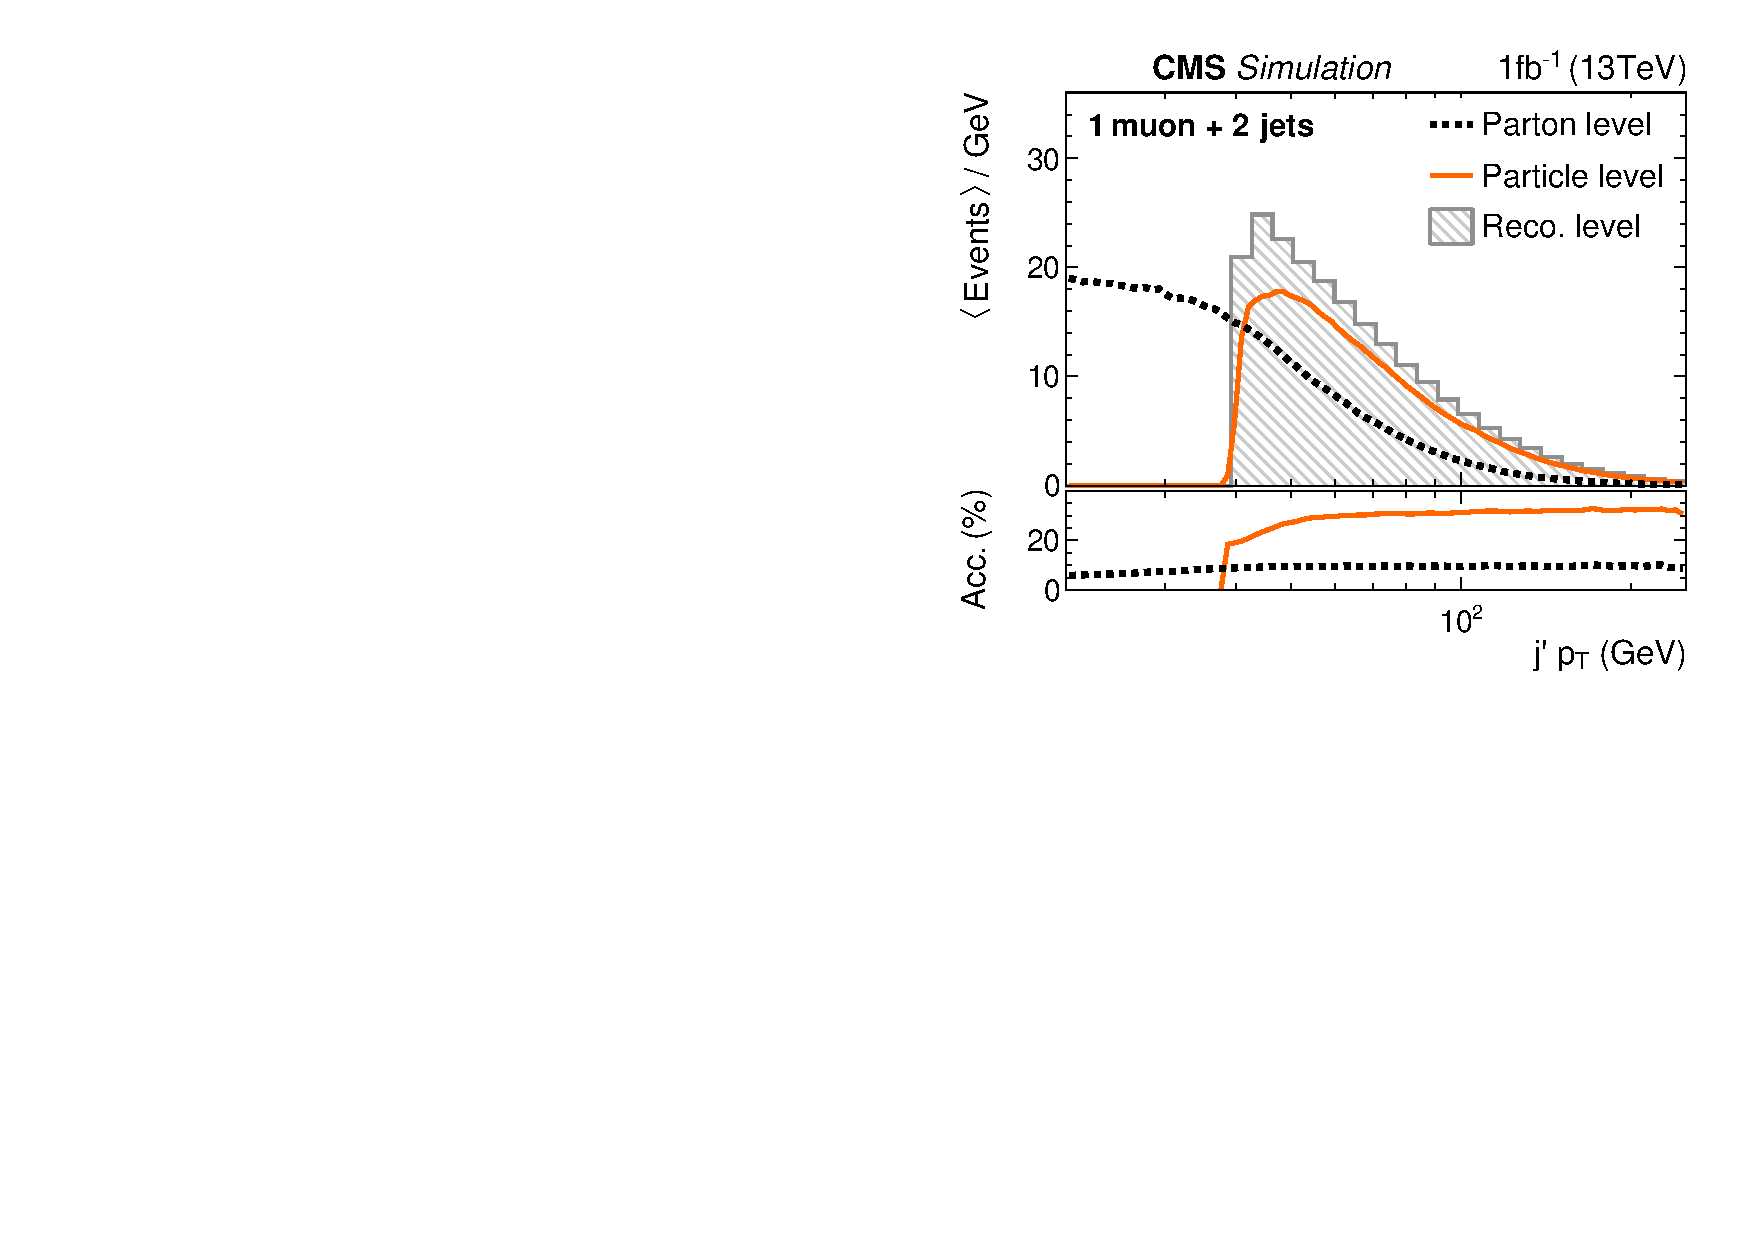
\includegraphics[width=0.48\textwidth]{figures/prospects/fiducial/ljet_particle_logpt.pdf}}\hspace{0.03\textwidth}
\subfloat[\label{fig:prospects-particle-level-ljeteta}]{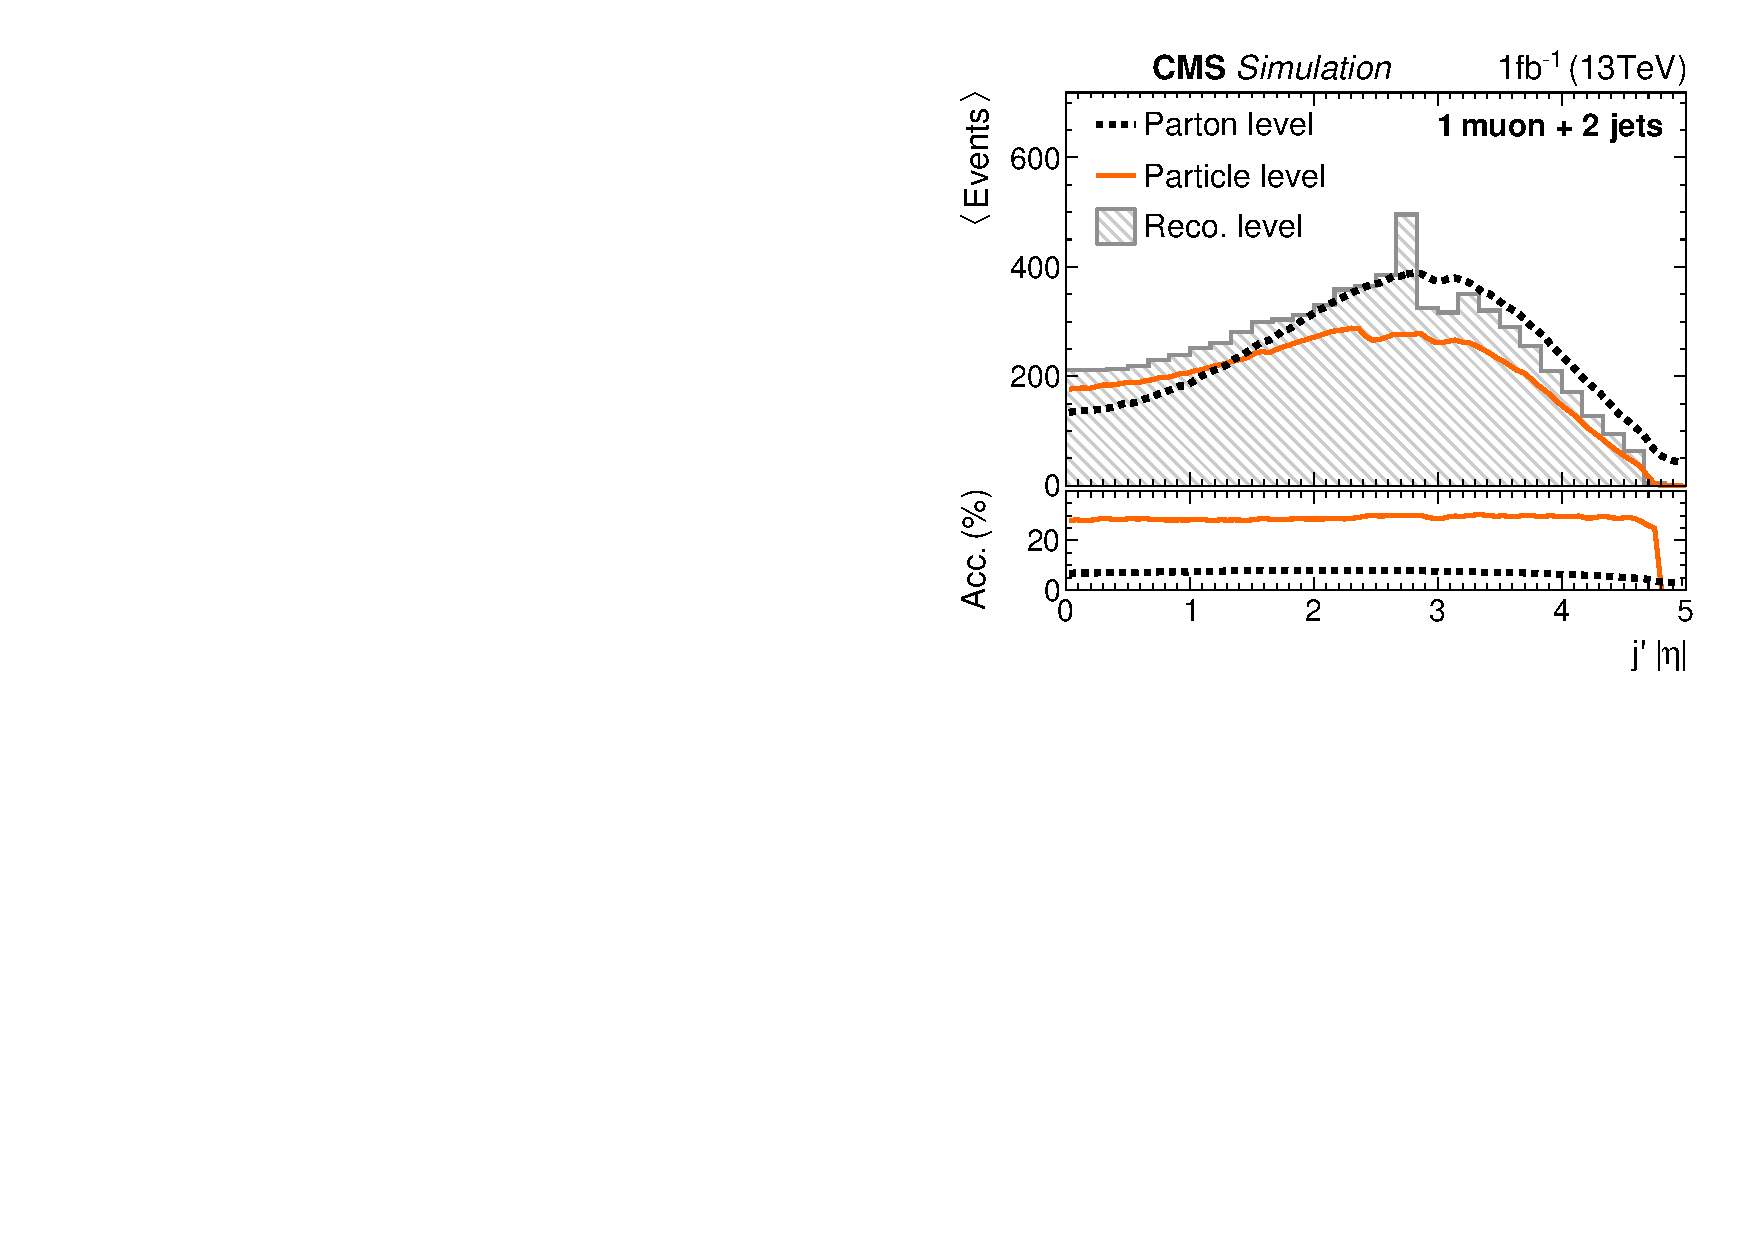
\includegraphics[width=0.48\textwidth]{figures/prospects/fiducial/ljet_particle_eta.pdf}}
}

\myfigure[phtb]{\label{fig:prospects-particle-top}Comparison of event selection at reconstruction and particle level.}{
\subfloat[]{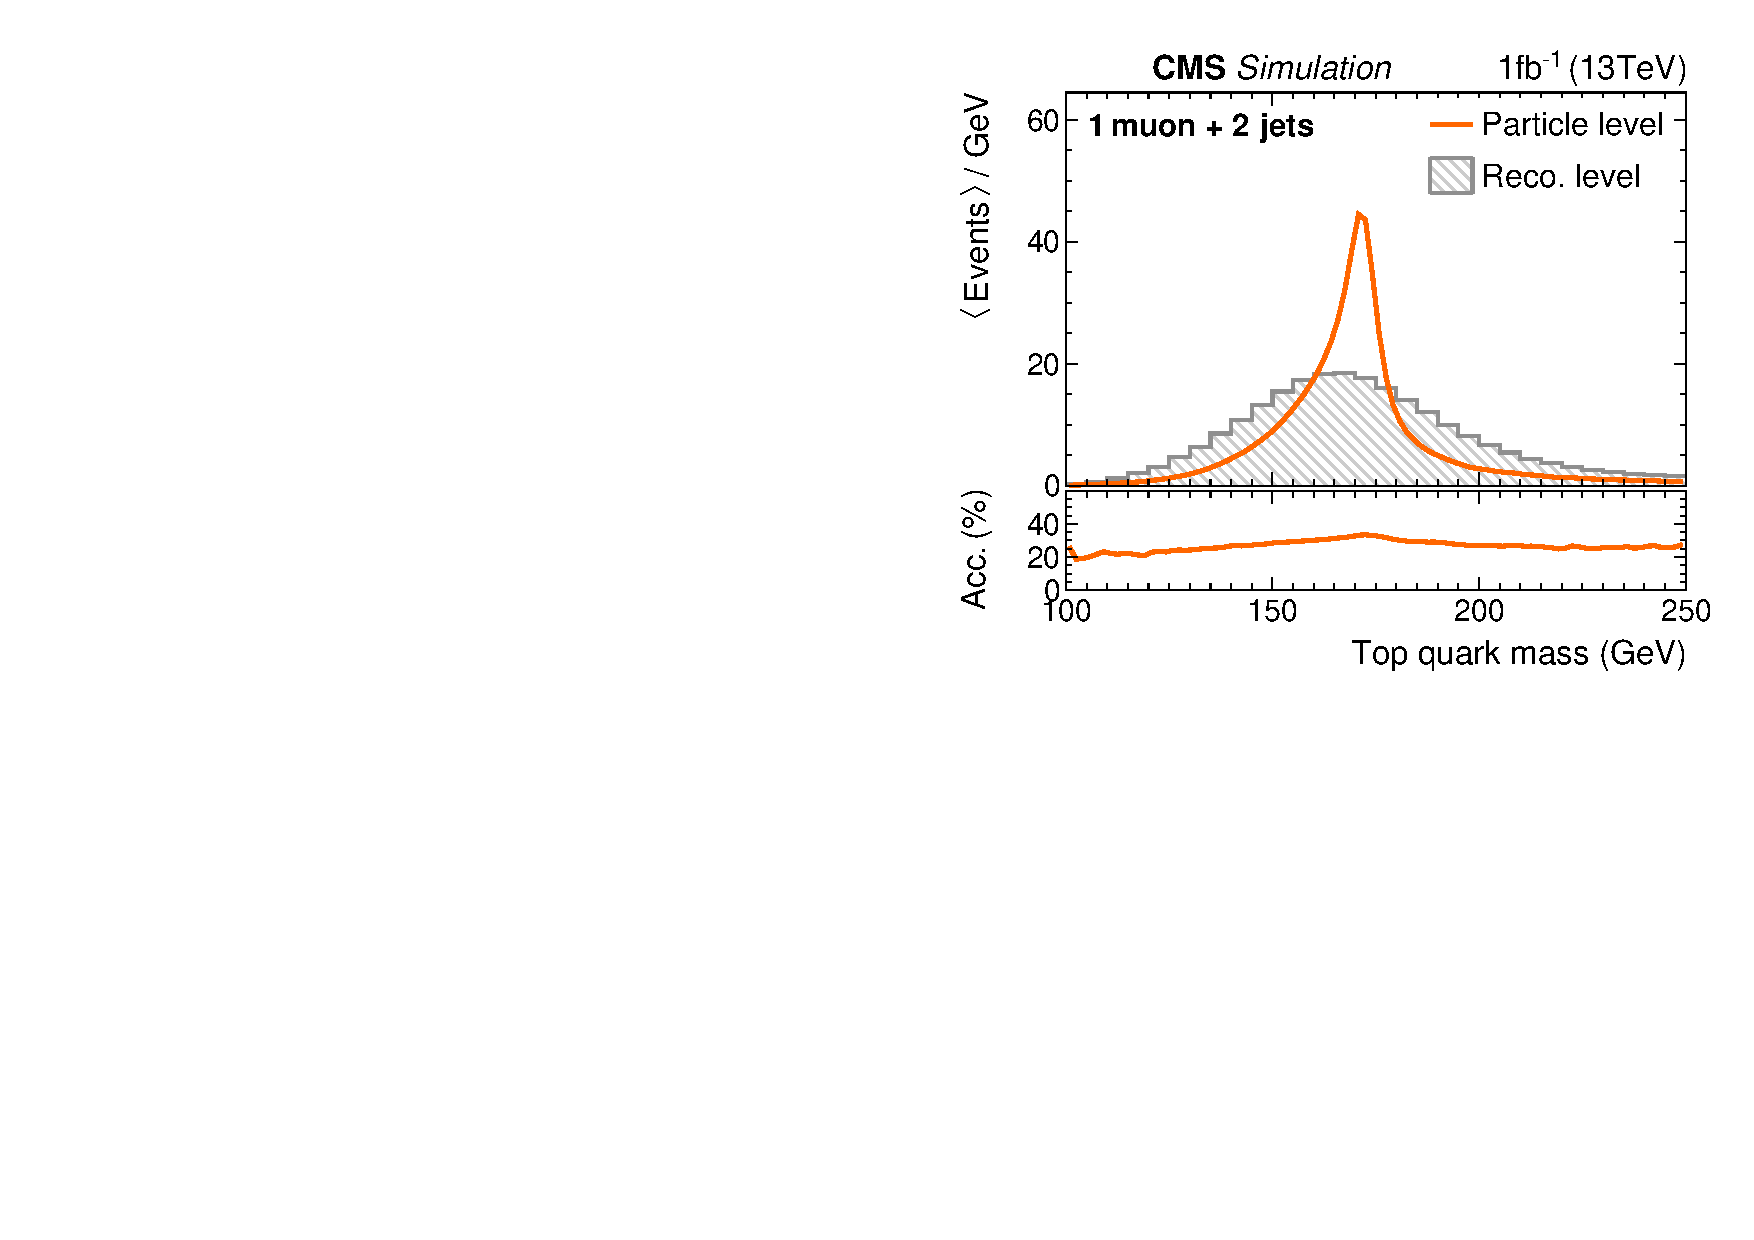
\includegraphics[width=0.48\textwidth]{figures/prospects/fiducial/top_particle_mass.pdf}}\hspace{0.03\textwidth}
\subfloat[]{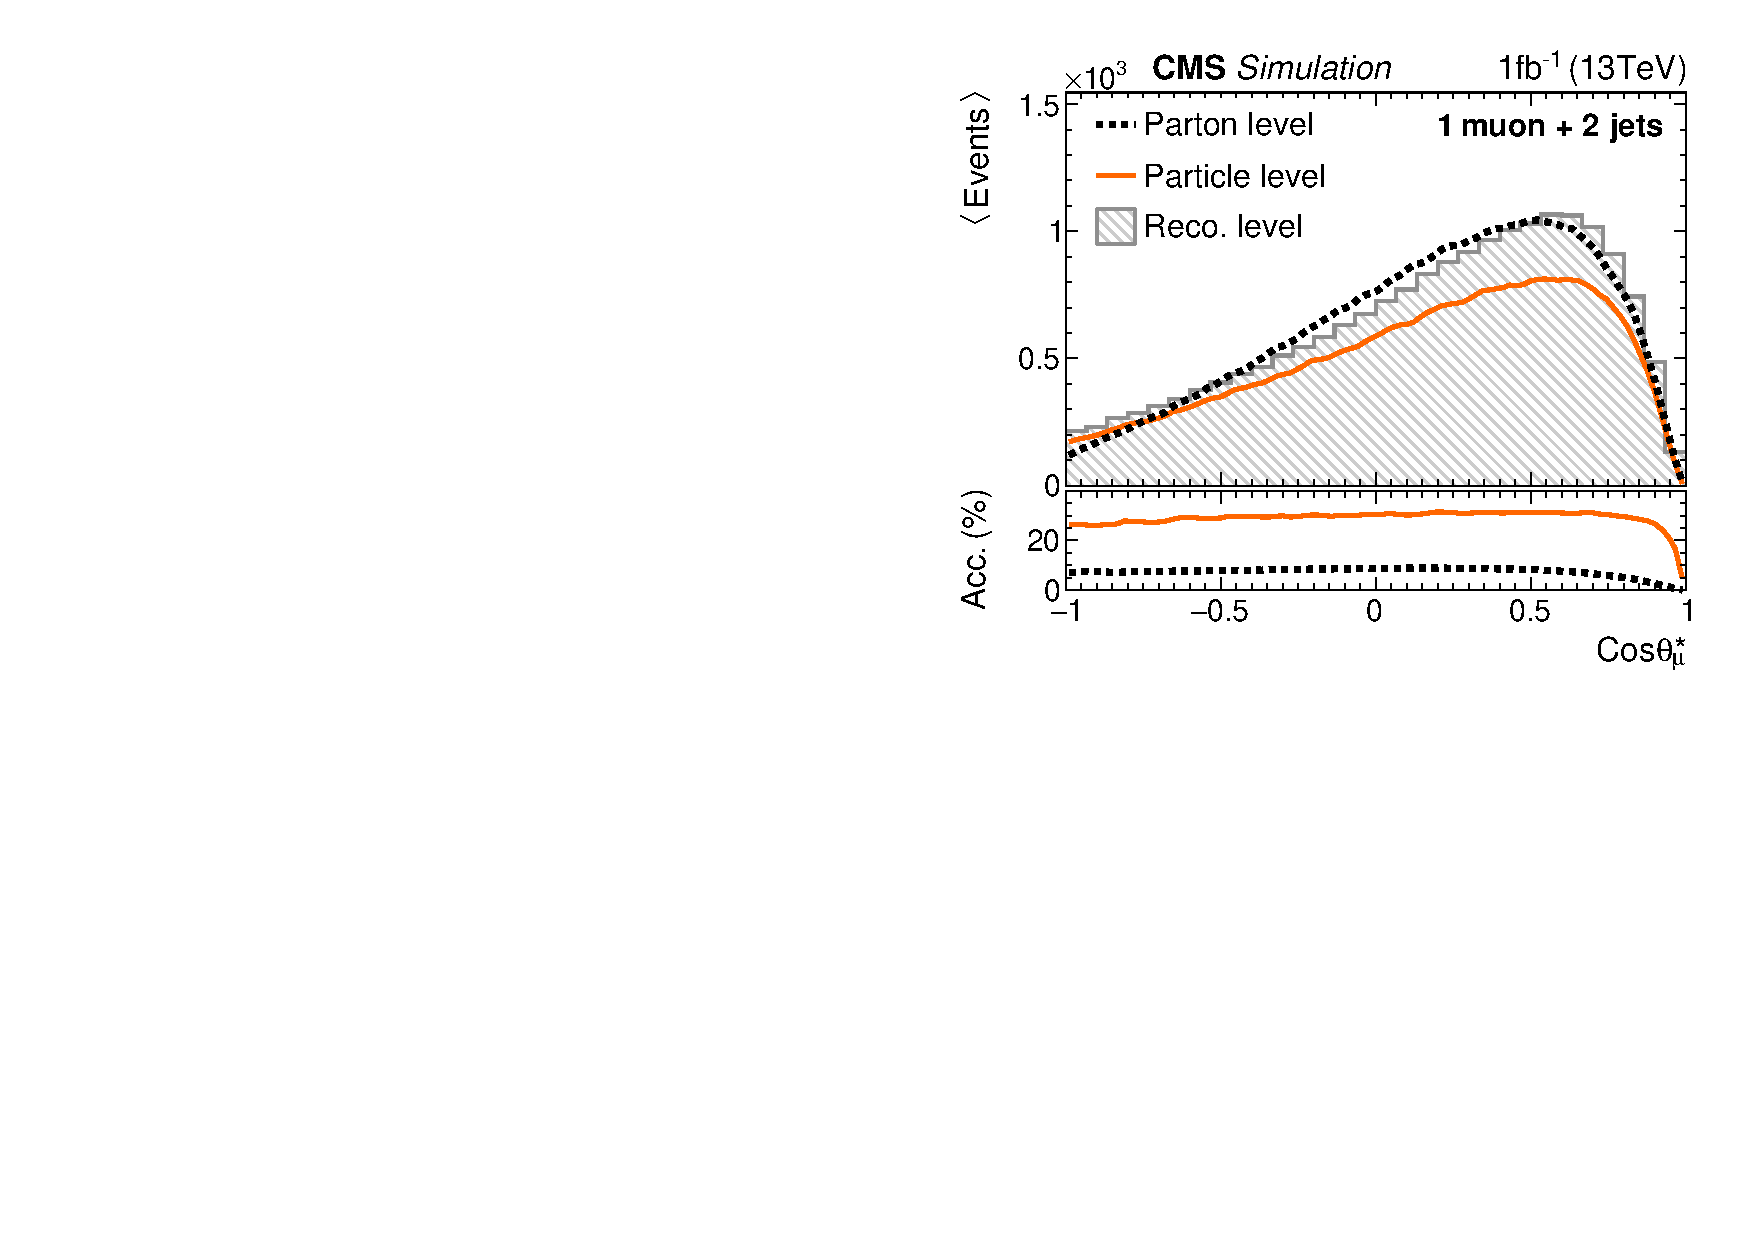
\includegraphics[width=0.48\textwidth]{figures/prospects/fiducial/cosTheta_particle.pdf}}
}

%############################################## 
\section{Validation}
%############################################## 

\myfigure[p]{\label{fig:pospects-validation}Validation in 2j1t control region (defined by $\bdttch<0$) of distributions in the (left column)~electron and (right column)~muon channel  .}{
\subfloat[]{\adjincludegraphics[height=4.8cm,trim={0 0 {0.16\width} 0},clip]{figures/prospects/plots/2j1t/electron_2j1t_top_pt_CR_nol.pdf}}
\subfloat[]{\adjincludegraphics[height=4.8cm,trim={0 0 {0.\width} 0},clip]{figures/prospects/plots/2j1t/muon_2j1t_top_pt_CR.pdf}}\\
\subfloat[]{\adjincludegraphics[height=4.8cm,trim={0 0 {0.16\width} 0},clip]{figures/prospects/plots/2j1t/electron_2j1t_top_absy_CR_nol.pdf}}
\subfloat[]{\adjincludegraphics[height=4.8cm,trim={0 0 {0.\width} 0},clip]{figures/prospects/plots/2j1t/muon_2j1t_top_absy_CR.pdf}}\\
\subfloat[]{\adjincludegraphics[height=4.8cm,trim={0 0 {0.16\width} 0},clip]{figures/prospects/plots/2j1t/electron_2j1t_cosTheta_tPL_CR_nol.pdf}}
\subfloat[]{\adjincludegraphics[height=4.8cm,trim={0 0 {0.\width} 0},clip]{figures/prospects/plots/2j1t/muon_2j1t_cosTheta_tPL_CR.pdf}}
}

%##############################################
\subsection{Excepted results on pseudo-data}
%##############################################